\documentclass[10pt,a4paper]{article}

\bibliographystyle{ieeetr}

\usepackage[margin=1in]{geometry}
\usepackage{graphicx}
\usepackage{subfig}
\usepackage{amsmath}
\usepackage{url}
\usepackage{pgfgantt}
\usepackage{pdfpages}
\usepackage[title]{appendix}

\graphicspath{{./figs/}}

\newcommand{\code}[1]{\texttt{#1}}

\begin{document}

\begin{titlepage}
    \begin{center}

        \vspace*{2cm}
        
\includegraphics[width=.25\textwidth]{crest.png}

        \vspace*{1cm}
        {\Large \textbf{An Educational Kernel for the Raspberry Pi}} \\

        \vspace*{1cm}
        \textbf{Thomas Archbold} \\
        1602581 \\
        Department of Computer Science \\
        University of Warwick \\~\\


        April 29, 2019 \\~\\

        CS310 Project \\
        supervised by Adam Chester \\~\\

        \vfill

    \end{center}
\end{titlepage}

% abstract
% 1. Purpose
% 2. Methodology/Project Design 
% 3. Findings/Contribution
% 4. Research Limitations/Future work
% 5. Practical Implications/Conclusions

% No jargon - understand all terms without additional reading
\begin{abstract}
    This project presents an educational operating system for the Raspberry Pi 1
    Model B+, written for the purpose of demystifying aspects of operating
    systems development for the hobbyist programmer, especially with regards to
    low-level systems programming and core features to a computer's execution.
    It provides a small multiprocessing kernel developed with the aim of clarity
    of understanding and ease of extension. Together with a simple interface to
    further configure the system at compile-time, it aims to promote a practical
    approach to operating systems education. This interface can be easily
    extended to accommodate different models of inter-process communication.
    Future work should be aimed at increasing the operating system's usability
    in a real-world context, in particular with regard to user input and access
    to permanent storage, of which it has none. While it is limited in this
    sense, it provides a simple and open testbed on which to both study how key
    operating system concepts are implemented in practice, as well as invite the
    addition of new features.
\end{abstract}


\tableofcontents

\section{Introduction}
    Operating systems are some of the most pervasive pieces of software around,
    but due to their inherent complexity, their inner workings are often
    impenetrable to understand without specialist knowledge. While widespread
    access to a personal computer is nothing new, the introduction of the
    Raspberry Pi in recent years has rendered experimentation with computers
    much more affordable and hence readily available, inviting tinkering at all
    levels with less concern of economic loss. The Pi therefore provides an
    ideal platform for operating systems education -- novice developers looking
    to get involved in writing such systems have access to a standardised set of
    hardware that is inexpensive both to maintain and replace, if and when
    things go wrong. Now seven years since its initial release, the Raspberry
    Pi has several official operating systems to offer, each addressing its own
    issue such as ease-of-installation, Internet of Things integration, or
    classroom management \cite{OSes}, with many more unofficial ones. However,
    there is less in the way of those written to teach concepts of the operating
    system itself -- this project attempts to fill this gap by providing a
    configurable, educational operating system for the Raspberry Pi 1 Model B+,
    with a focus on presenting code which is simple to understand and providing
    clear interfaces to encourage ease of extensibility, and hence a practical,
    software-driven approach to learning about operating systems.

\subsection{Useful concepts}

\input{sections/conclusions}

\bibliography{bibliography}

%\begin{appendices}
%
%    \pagenumbering{gobble}
%
%    % Revised Timetable
%    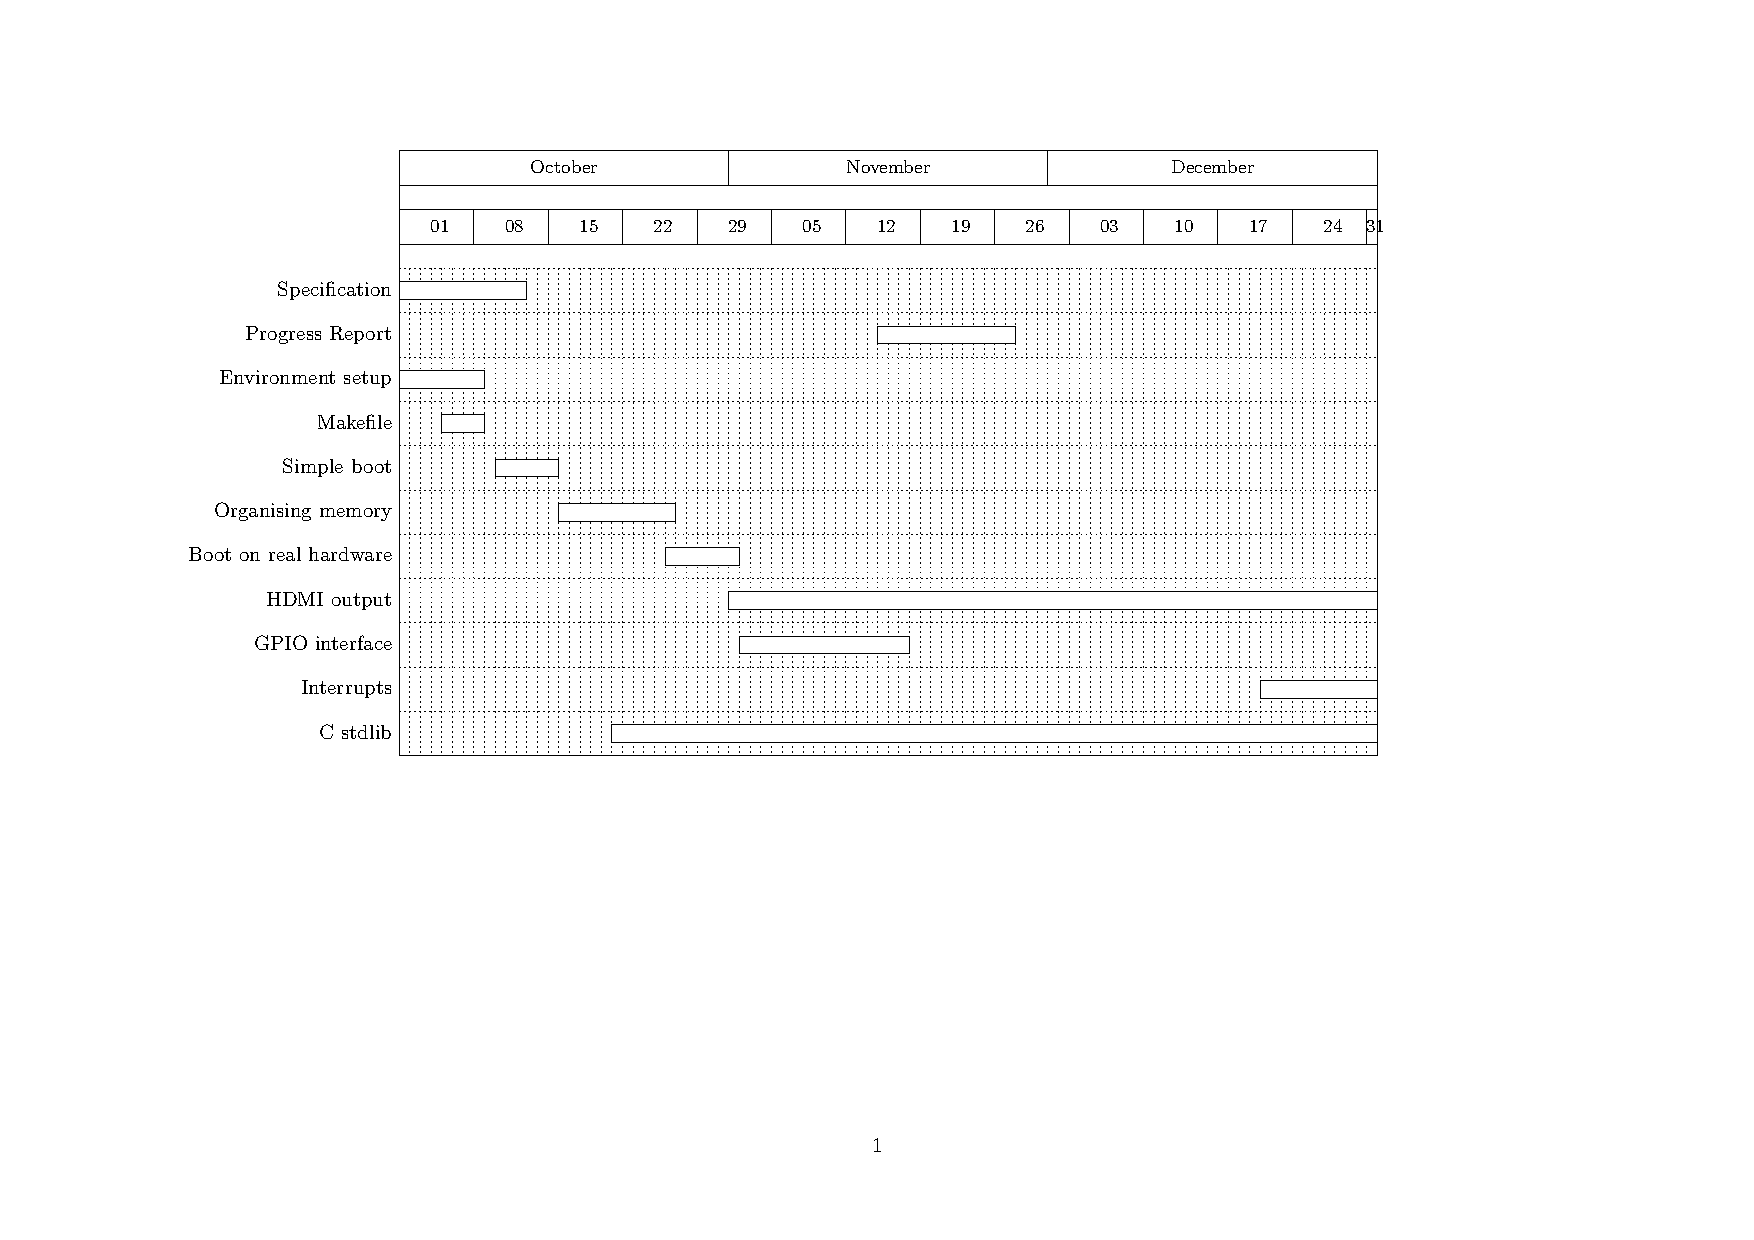
\includepdf[landscape=true,pages=1,pagecommand={\section{Revised Timetable}}]{timetable/timetable.pdf}
%    \includepdf[landscape=true,pages=2,pagecommand={}]{timetable/timetable.pdf}
%
%    % Project Specification
%    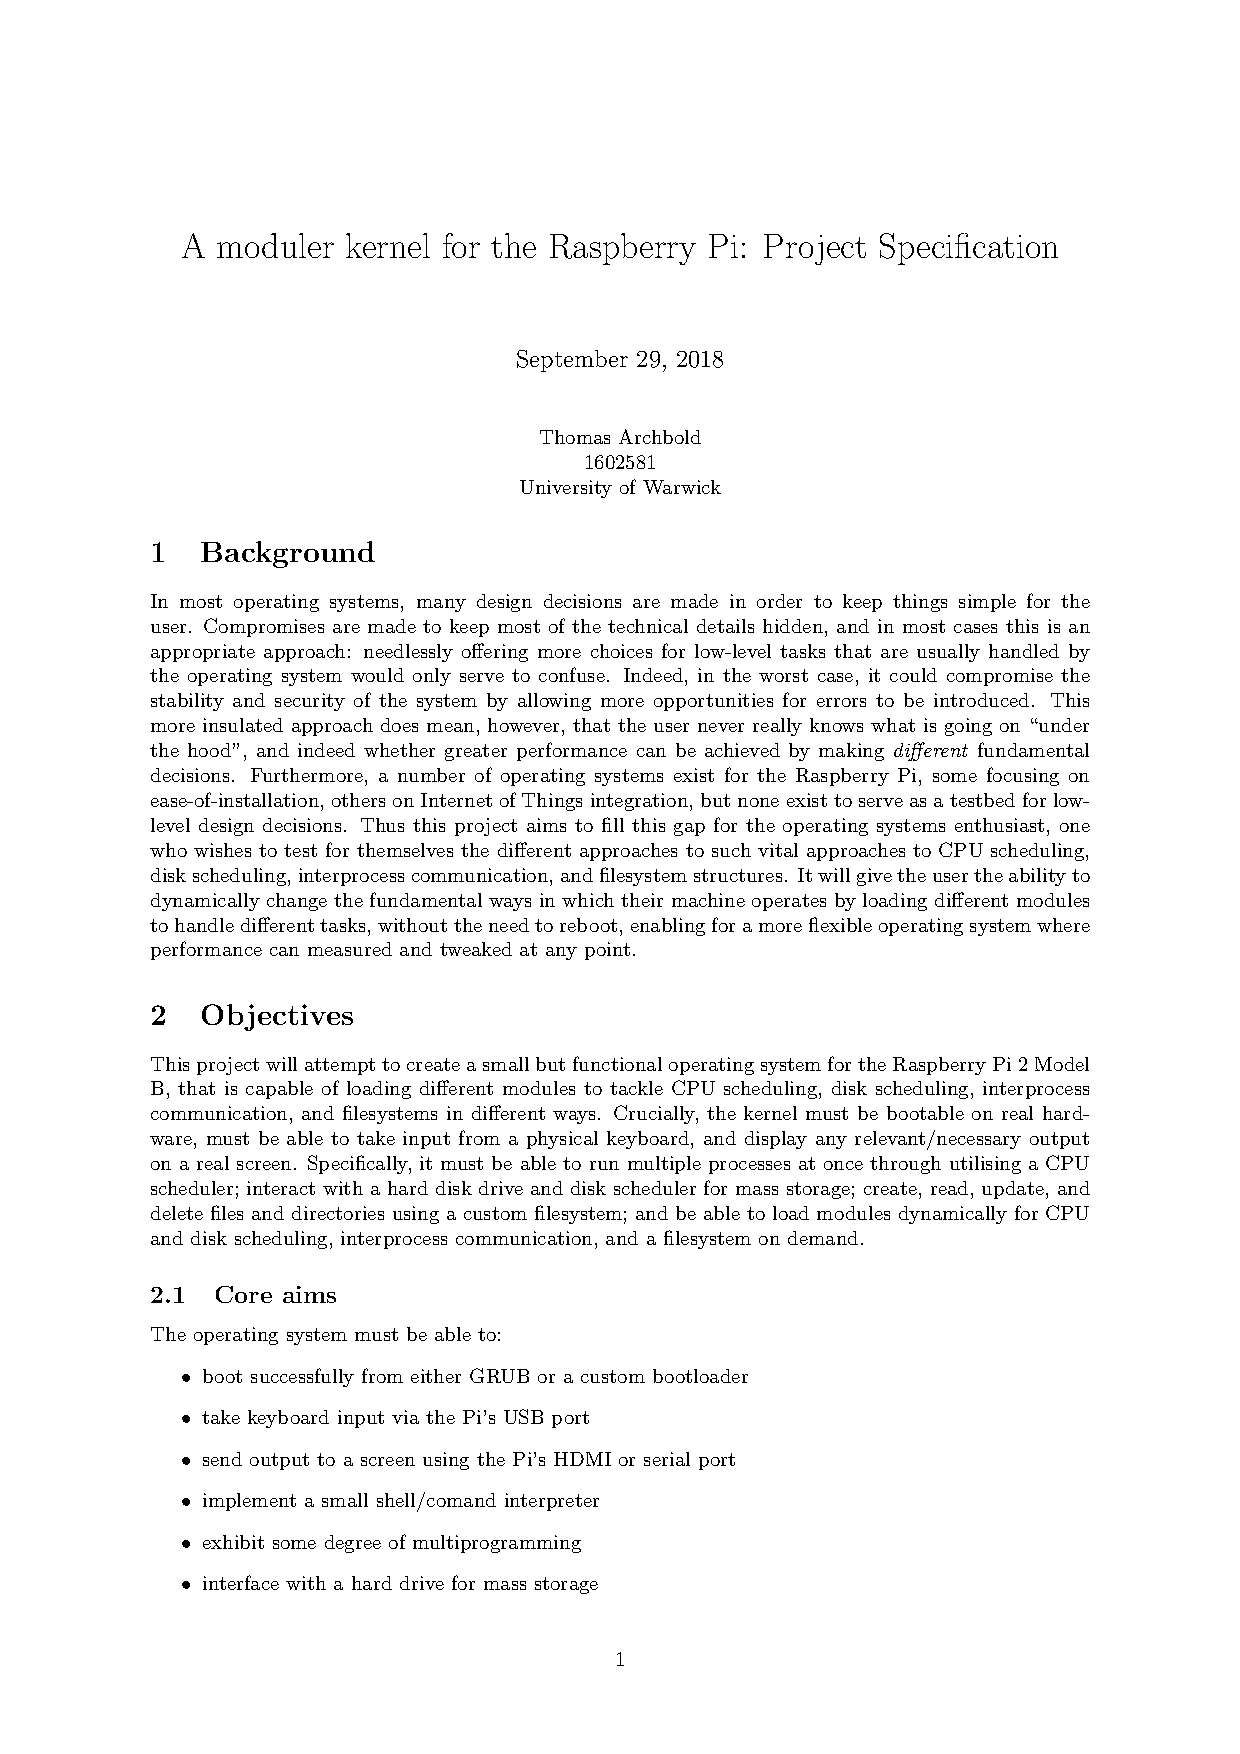
\includepdf[pages=1,pagecommand={\section{Project Specification}}]{../specification/specification.pdf}
%    \includepdf[pages=2-6,pagecommand={}]{../specification/specification.pdf}
%    \includepdf[landscape=true,pages=7-,pagecommand={}]{../specification/specification.pdf}
%
%\end{appendices}

\end{document}
